\documentclass{beamer}
\usepackage{beamerthemesplit}

%Seitenzahlen
\newcommand*\oldmacro{}%
\let\oldmacro\insertshorttitle%
\renewcommand*\insertshorttitle{%
  \oldmacro\hfill%
  \insertframenumber\,/\,\inserttotalframenumber}

\setbeamertemplate{caption}{\raggedright\insertcaption\par}

%Definieren uns farbigen Quellcode
\usepackage{color}
\definecolor{dkgreen}{rgb}{0,0.6,0}
\definecolor{gray}{rgb}{0.5,0.5,0.5}
\definecolor{mauve}{rgb}{0.58,0,0.82}
 
%Damit wir Quellcode nutzen können.
\usepackage{listings}
\lstset{numbers=left,
	numberstyle=\tiny,
	numbersep=5pt,
	breaklines=true,
	showstringspaces=false,
	frame=l ,
	xleftmargin=15pt,
	xrightmargin=15pt,
	basicstyle=\ttfamily\scriptsize,
	stepnumber=1,
	keywordstyle=\color{blue},          % keyword style
  	commentstyle=\color{dkgreen},       % comment style
  	stringstyle=\color{mauve}         % string literal style
}
%Sprache Festelegen
\lstset{language=C++}

\begin{document}
\title{Infinite Impulse Response Filters} 
\author{Judith Massa, Patrick Esser}
\date{\today} 

\frame{\titlepage} 
\frame{\frametitle{Overview}\tableofcontents[hideallsubsections]} 

\section{Motivation}
\subsection{Ilastik}
\frame{\frametitle{Ilastik}
\begin{figure}
\begin{tabular}{c}
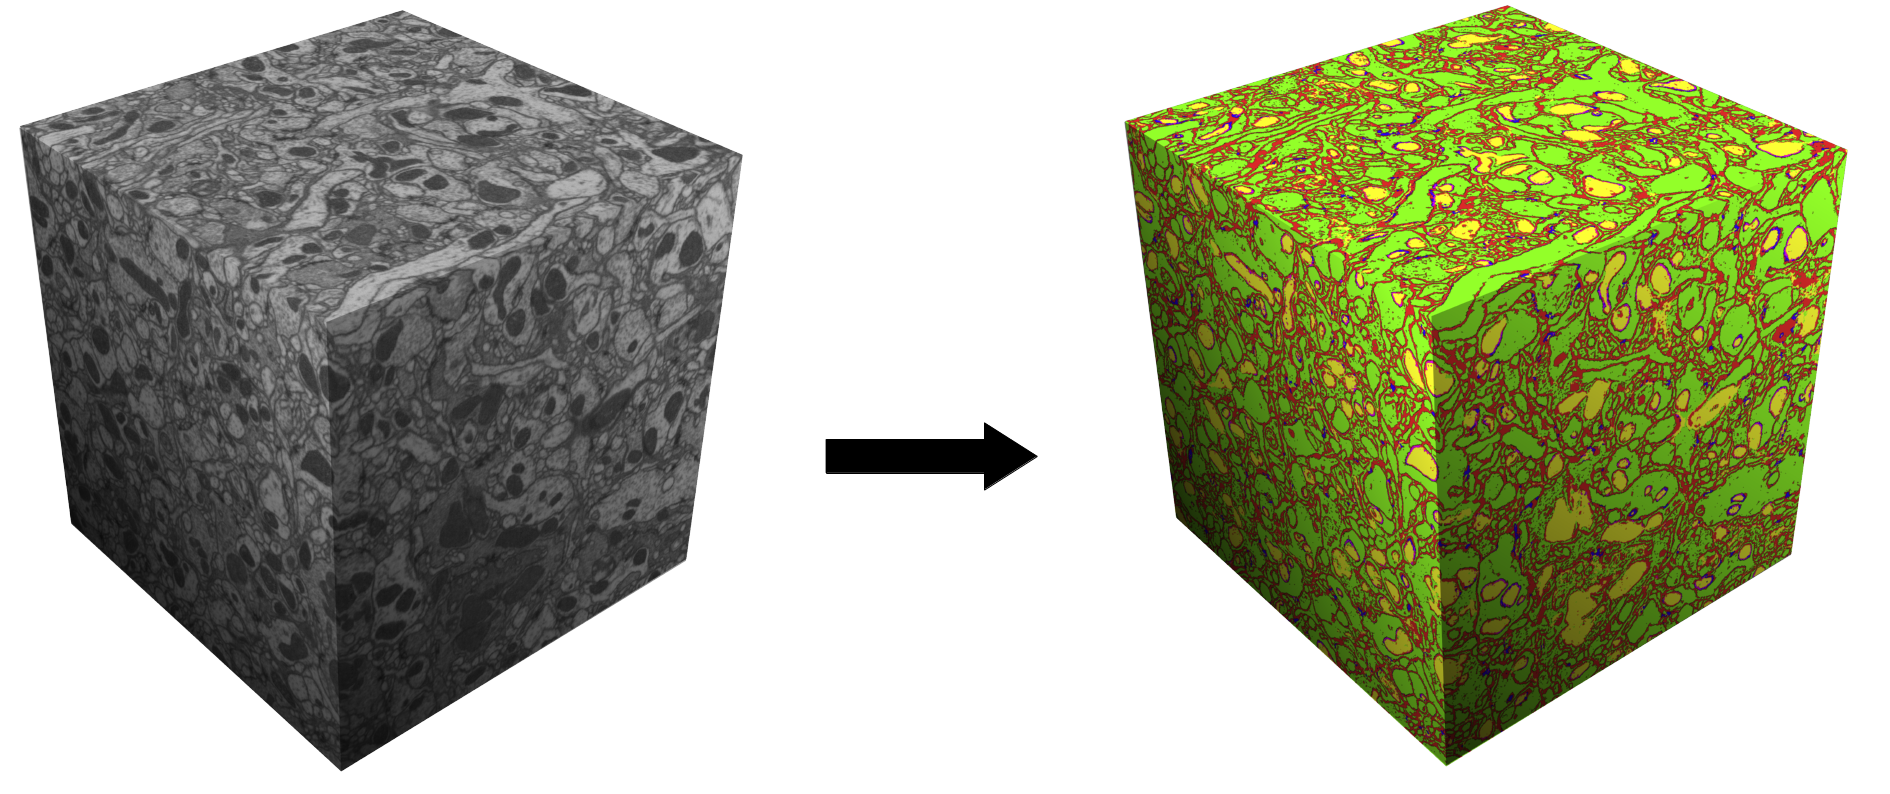
\includegraphics[scale=0.1]{imgs/cubes_combined.jpg}
\end{tabular}
\end{figure}
\begin{itemize}
  \item Ilastik: toolkit for interactive image classification and segmentation
  \item Algorithms rely on precomputed features of the image
\end{itemize}
\begin{figure}
\centering
\begin{tabular}{ccc}
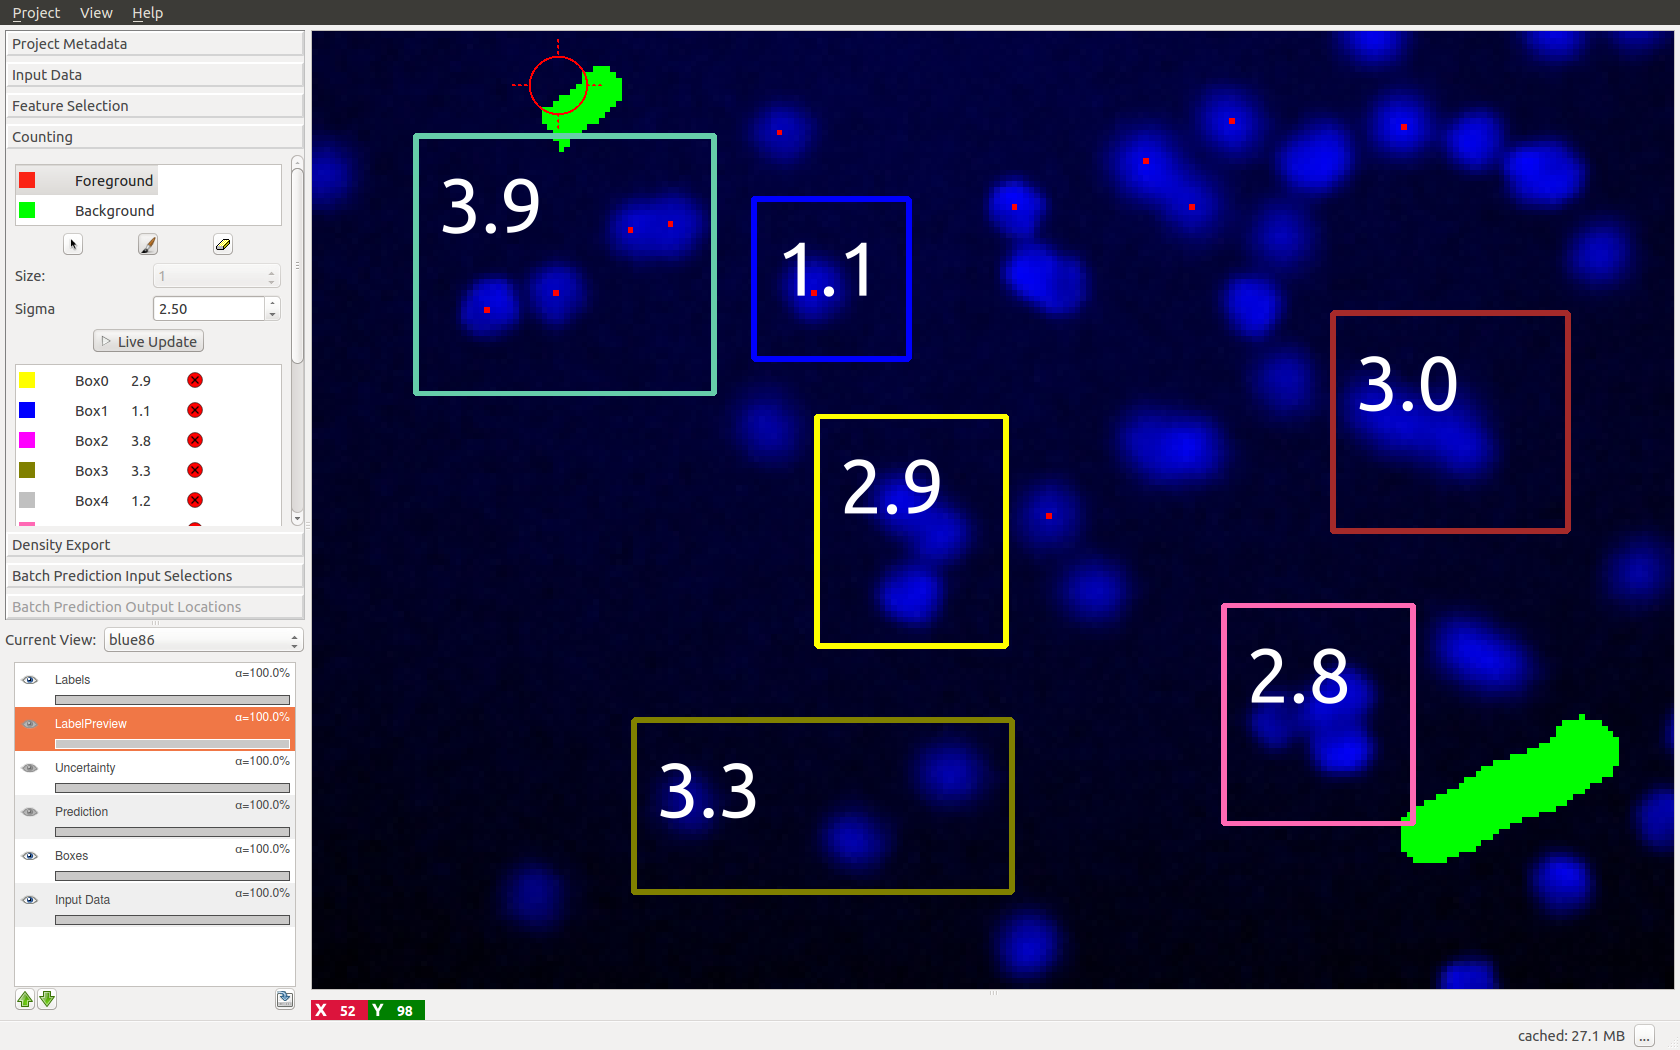
\includegraphics[scale=0.05]{imgs/ilastik1.png}\quad &
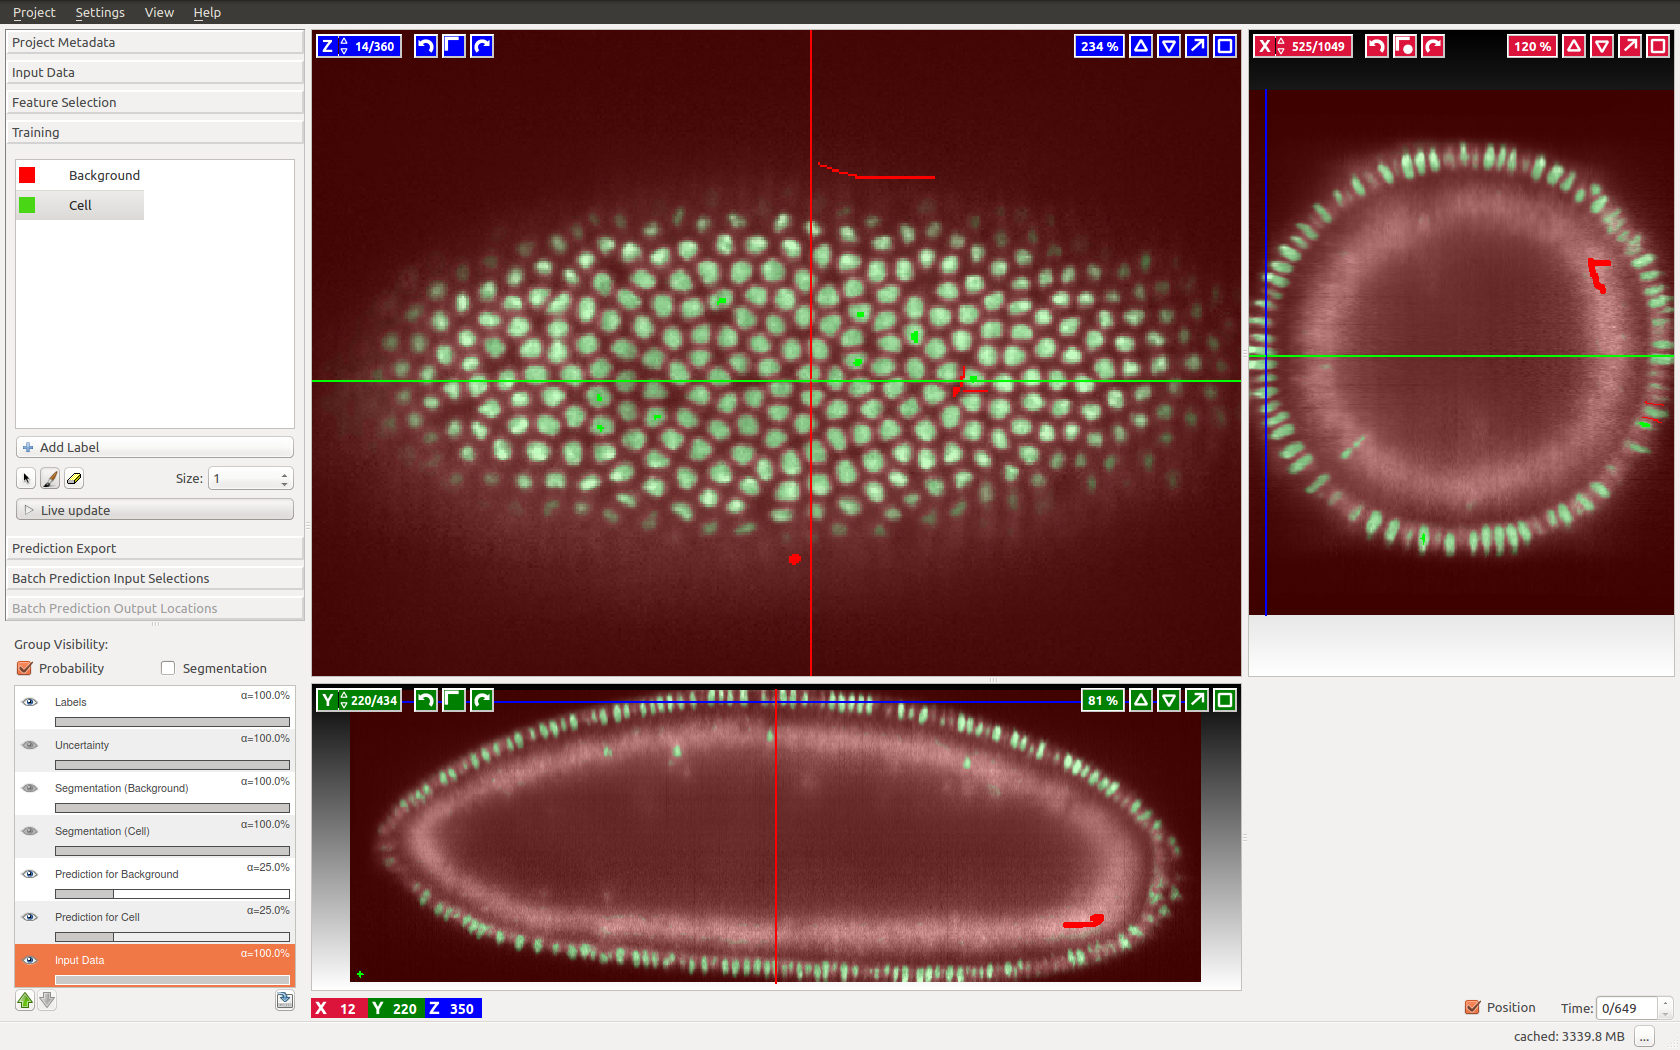
\includegraphics[scale=0.05]{imgs/ilastik2.png}\quad &
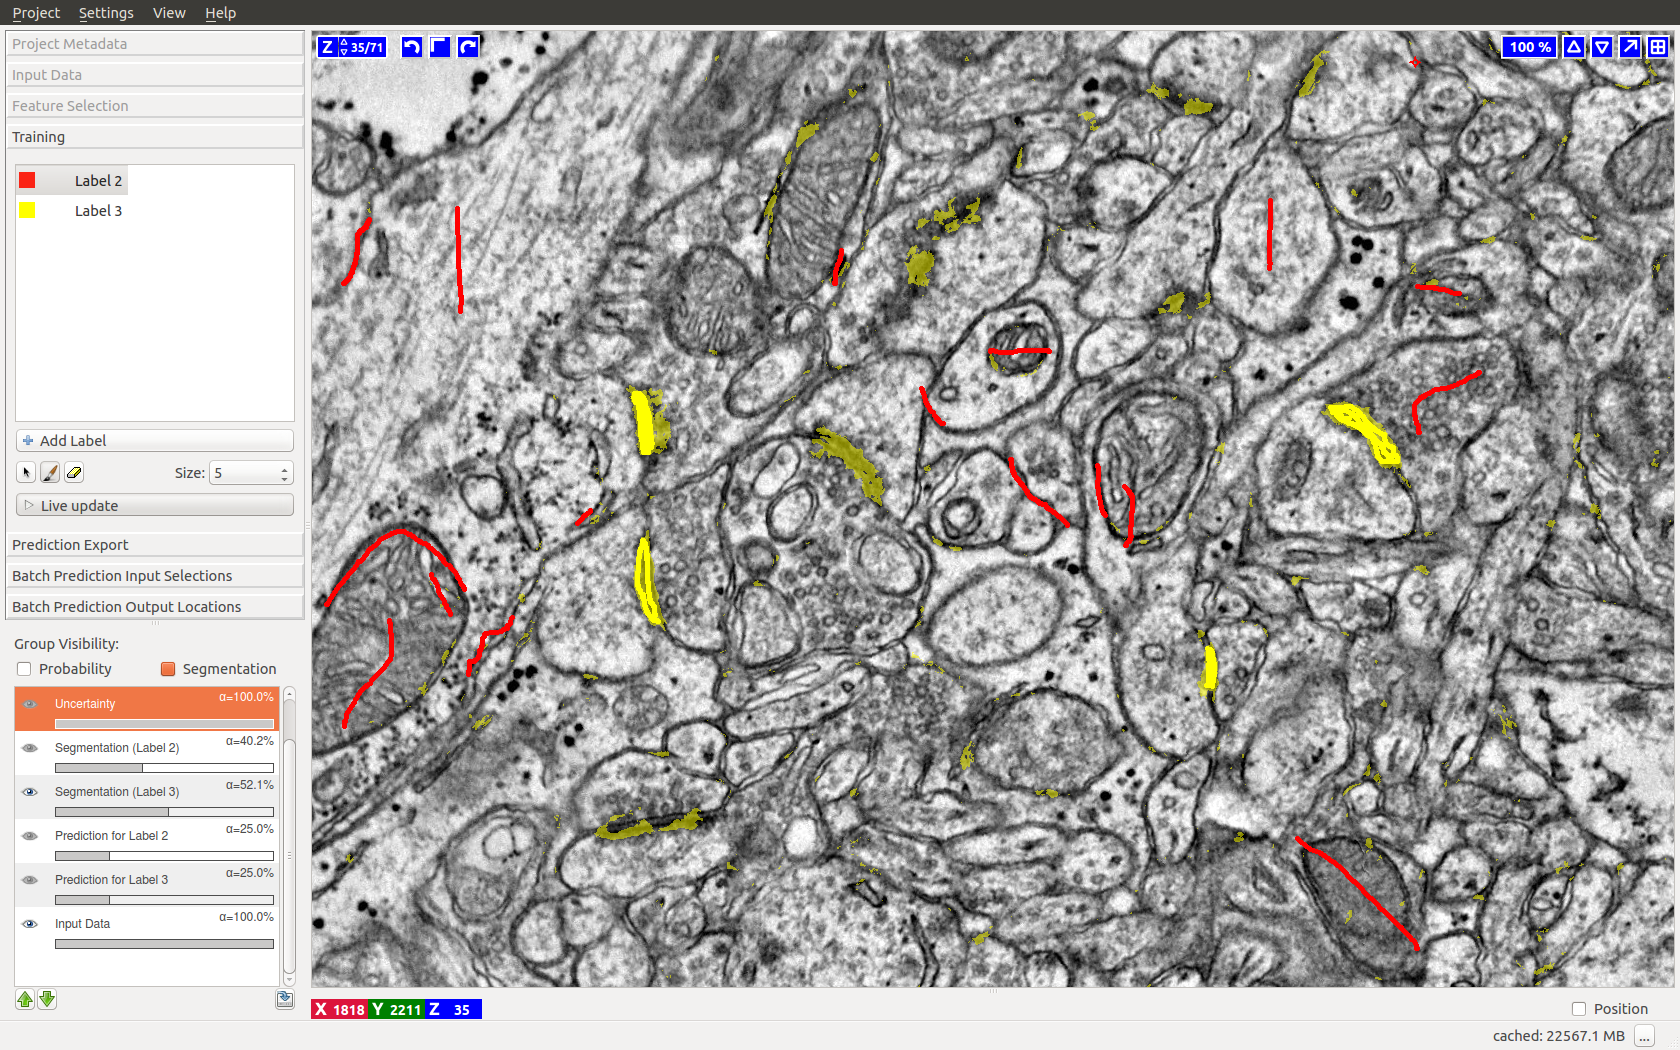
\includegraphics[scale=0.07]{imgs/ilastik3.png} 
\end{tabular}
\end{figure}
}

\frame{\frametitle{Tracking}
\begin{itemize}
  \item Project supervisor Sven Peter is working on object tracking \\
        $\to$ Requires classification scale space and edge detection
  \item Tracking example:
\end{itemize}

\begin{figure}
\centering
\begin{tabular}{cc}
\includegraphics[scale=0.08]{imgs/tracking1.png}\quad &
\includegraphics[scale=0.08]{imgs/tracking2.png} 
\end{tabular}
\caption{Application in Biology: Cell Tracking}
\end{figure}
}

\subsection{Gaussian Filtering}
\frame{\frametitle{Gaussian Filtering}
Convolution: 
$$(f*g)(x) := \int_{\mathbb{R}^n} f(x-y)g(y)\mathrm{d}y$$
\begin{itemize}
  \item discrete: $(f*g)(x)=\sum_{y=-\infty}^\infty f(x-y)\, g(y)$
  \item $f\ldots$ image
  \item $g\ldots$ filter, e.g. Gaussian
\end{itemize}

Gaussian:
\begin{itemize}
  \item $g=\frac{1}{\sqrt{2\sigma^2\pi}}e^{-{\frac {(x-\mu)^{2}}{2\sigma^{2}}}}$
  \item Convolution with Gaussian gives scale space representations
  \item Convolution with Gaussian derivative gives derivative of smoothed
    image (edge features)
\end{itemize}
}

\subsection{Implementations of Filters}
\frame{\frametitle{Implementations of Filters}
\begin{itemize}
  \item Finite Impulse Response Filters (FIR):
  \begin{itemize}
  \item if $g$ finite (with $2M+1$ entries):
  $$(f*g)(x)=\sum_{y=-\infty}^\infty f(x-y)\, g(y) = \sum_{y=-M}^M f(x-y)g(y)$$
  \item multiple muliply-adds for one pixel
   \end{itemize}
  \item Fast Fourier Transform (FFT)
  \begin{itemize}
  \item $\mathcal{F}(f)(\omega) = 
      \int_{\mathbb{R}^n} f(x)\,e^{-\mathrm{i}\omega x2\pi} \,\mathrm{d} x$
  \item discrete and finite: $\mathcal{F}(f)(\omega) = \sum_{x=0}^{N-1} f(x) \cdot e^{- \mathrm{i}\omega x \frac{2\pi}{N}}$
  $f(x) = \frac{1}{N}\sum_{\omega=0}^{N-1} \mathcal{F}(f)(\omega) \cdot e^{- \mathrm{i}\omega x \frac{2\pi}{N}}\qquad
      \text{\small{($N\ldots$ number of pixels)}}$
  $$(f*g)(x) = \left(\mathcal{F}^{-1}\mathcal{F}(f*g)\right)(x)
      = (\mathcal{F}^{-1}[\underbrace{\mathcal{F}(g)}_{\text{precomputed}}\cdot\,\mathcal{F}(f)])(x)$$
  \item after transformation 1 multiplication per pixel
  \end{itemize}
\end{itemize}
}

\frame{\frametitle{Implementations of Filters}
Problems:
\begin{itemize}
  \item suffer from increasing stencils
  \begin{itemize}
  \item e.g. wide Gaussian (needed for coarse-scale representation) 
  \end{itemize}
  \item FFT does not always outperform FIR on GPUs \cite{1648322}
\end{itemize}
Alternative: Infinite Impulse Response Filters (IIR)
}


\section{IIR}
\subsection{Idea}
\frame{\frametitle{IIR Filters}
Idea:
\begin{itemize}
  \item Instead of using possibly wide stencil \\
    $\to$ Approximate by a fixed size stencil and use recursion \\
    $\to$ Recursion makes filter infinite: \\
   \qquad all previous values taken into account
\end{itemize}
   $$y(i) = \sum_{k=0}^{N-1} n(i)x(i-k) - \sum_{k=1}^{D} d(k) y(i-k)$$
}

\subsection{Properties}
\frame{\frametitle{Properties}

\begin{itemize}
  \item Approximation error of IIR-filters: $\approx 10^{-4}$\\
    $\to$ single precision enough

  \item Computational cost does not depend on scale parameter\\
    $\to$ Cost is fixed, no filter comparison necessary

  \item Each row's column depends on previous column's result\\
    $\to$ Less parallelism than FIR
\end{itemize}
}

\subsection{Original Algorithm}
\begin{frame}
\frametitle{Causal and Anticausal pass}

\begin{itemize}
  \item Approximate a one dimensional, causal filter, i.e.
    \begin{equation}
      y_i = \sum_{k = 0}^{N-1} h_k x_{i - k}
    \end{equation}
  \item Split a one dimensional non causal filter,
    \begin{equation}
      y_i = \sum_{k = -M}^{M} h_k x_{i - k}
    \end{equation}
    into a causal and anticausal filter, i.e.
    \begin{equation}
      h^+_k = \begin{cases}
        h_k & k \ge 0 \\
        0 & k < 0
      \end{cases},
      \quad
      h^-_k = \begin{cases}
        0 & k \ge 0 \\
        h_k & k < 0
      \end{cases}
    \end{equation}
      
\end{itemize}
\end{frame}

\begin{frame}
\frametitle{Horizontal and Vertical pass}

\begin{itemize}
  \item Approximate those two (anti-)causal filters $\to$ Causal (left to
    right) and Anticausal (right to left) passes
  \item Extend to two dimensions: One filter per row (Horizontal pass) and
    one filter per column (Vertical pass)
\end{itemize}
  $\to$ total of $4$ passes: Left-to-right (causal) and right-to-left
    (anticausal) in each row (horizontal) and top-to-bottom (causal) and
    bottom-to-top (anticausal) in each column (vertical). Details in
    \cite{deriche}.
\end{frame}

\begin{frame}
\frametitle{Original Algorithm}

    \lstinputlisting[firstline=67, lastline=84, basicstyle=\tiny]{code/svenpeter_convolve_iir_nosimd.cxx}
\begin{itemize}
  \item $y_i = [x_i,\;x_{i-1},\;x_{i-2},\;x_{i-3}]\cdot\mathbf{n}
  - [y_{i-1},\;y_{i-2},\;y_{i-3},\;y_{i-4}]\cdot\mathbf{d}$ 
  \item Anticausal pass similar to causal 
\end{itemize}
\end{frame}

\begin{frame}
\frametitle{Border Treatment}

\begin{itemize}
  \item Mirroring: $[\ldots,\;x_{2},\;x_{1},\;x_0,\;x_{1},\;x_{2},\;x_{3},\;x_{4},\;x_{5},\;x_{6},\;x_{7},\;x_{8},\ldots]$
\end{itemize}
   \lstinputlisting[firstline=47, lastline=65, basicstyle=\tiny]{code/svenpeter_convolve_iir_nosimd.cxx}
\end{frame}

\section{Parallelization}
\subsection{Overview}
\frame{\frametitle{Possibilities and challenges}
\begin{enumerate}
  \item All rows (columns) independent in horizontal (vertical) pass
  \item Causal and anticausal pass independent
  \item Either horizontal or vertical pass will cause bad memory layout
  \item Parallelize recurrence relation within each row
  \item Compute multiple features for multiple images concurrently
\end{enumerate}
}

\subsection{Parallelizing over rows/columns}
\begin{frame}[fragile]
\frametitle{Causal pass}
  \begin{lstlisting}[basicstyle=\tiny]
thrust::for_each_n(
  thrust::counting_iterator<int>(0), height,
  [buffer_begin, src_begin, row_stride, column_stride, width, c]
  __device__ (int n) {
    auto row = buffer_begin + n * row_stride;
    auto src = src_begin + n * row_stride;
    // init recursion ... then recurse
    for(int i = 4; i < width; ++i)
    {
      row[i * column_stride] =
        c.b_causal[0] * src[(i - 0) * column_stride]
      + c.b_causal[1] * src[(i - 1) * column_stride]
      + c.b_causal[2] * src[(i - 2) * column_stride]
      + c.b_causal[3] * src[(i - 3) * column_stride]
      - c.a[1] * row[(i - 1) * column_stride]
      - c.a[2] * row[(i - 2) * column_stride]
      - c.a[3] * row[(i - 3) * column_stride]
      - c.a[4] * row[(i - 4) * column_stride];
    }
  });
  \end{lstlisting}
\end{frame}

\begin{frame}{Results}
  \begin{columns}
    \begin{column}{7cm}
      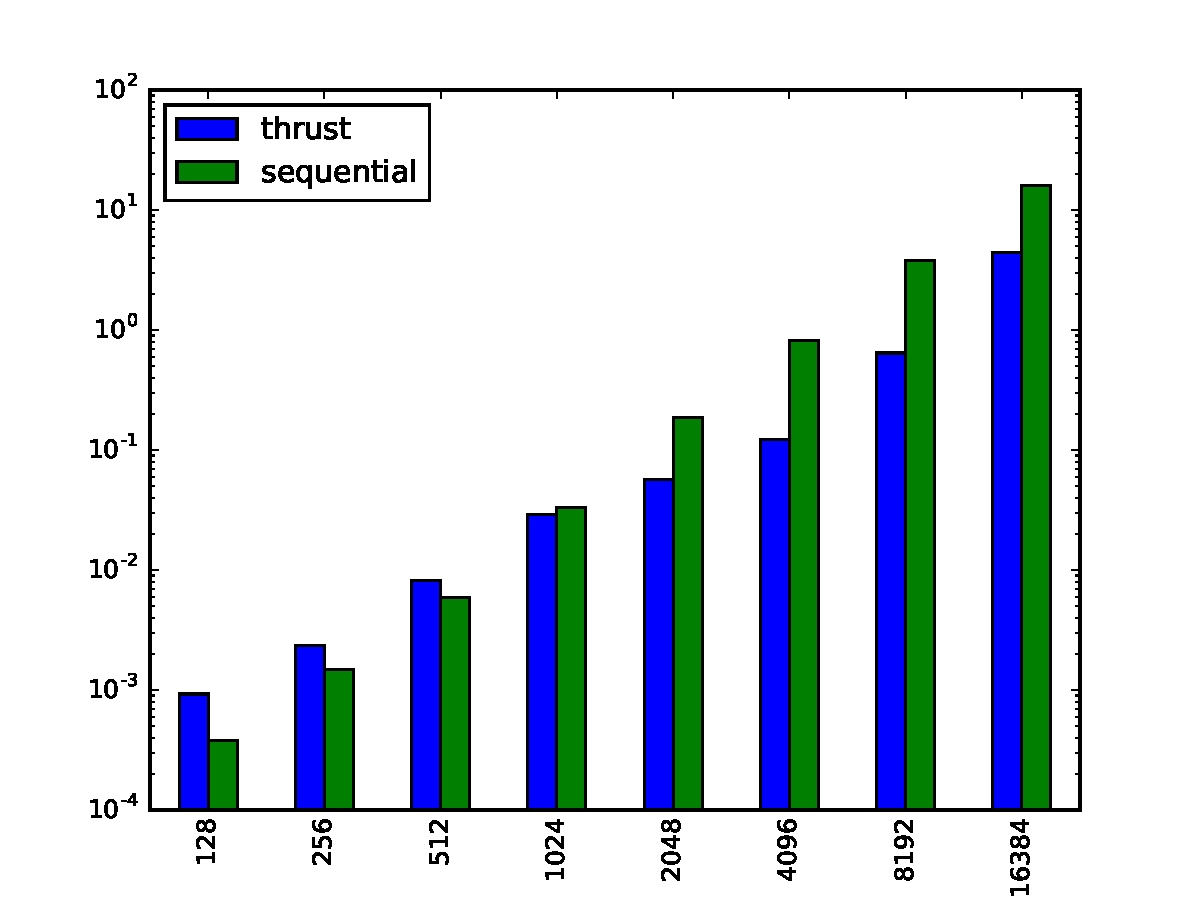
\includegraphics[scale=0.4]{imgs/thrust_vs_sequential_total.pdf} 
    \end{column}
    \begin{column}{3cm}
      \begin{itemize}
        \item code handles horizontal and vertical passes by adjusting
          strides
        \item results do not look very promising
      \end{itemize}
    \end{column}
  \end{columns}
\end{frame} 

\begin{frame}{A closer look}
  \begin{columns}
    \begin{column}{7cm}
      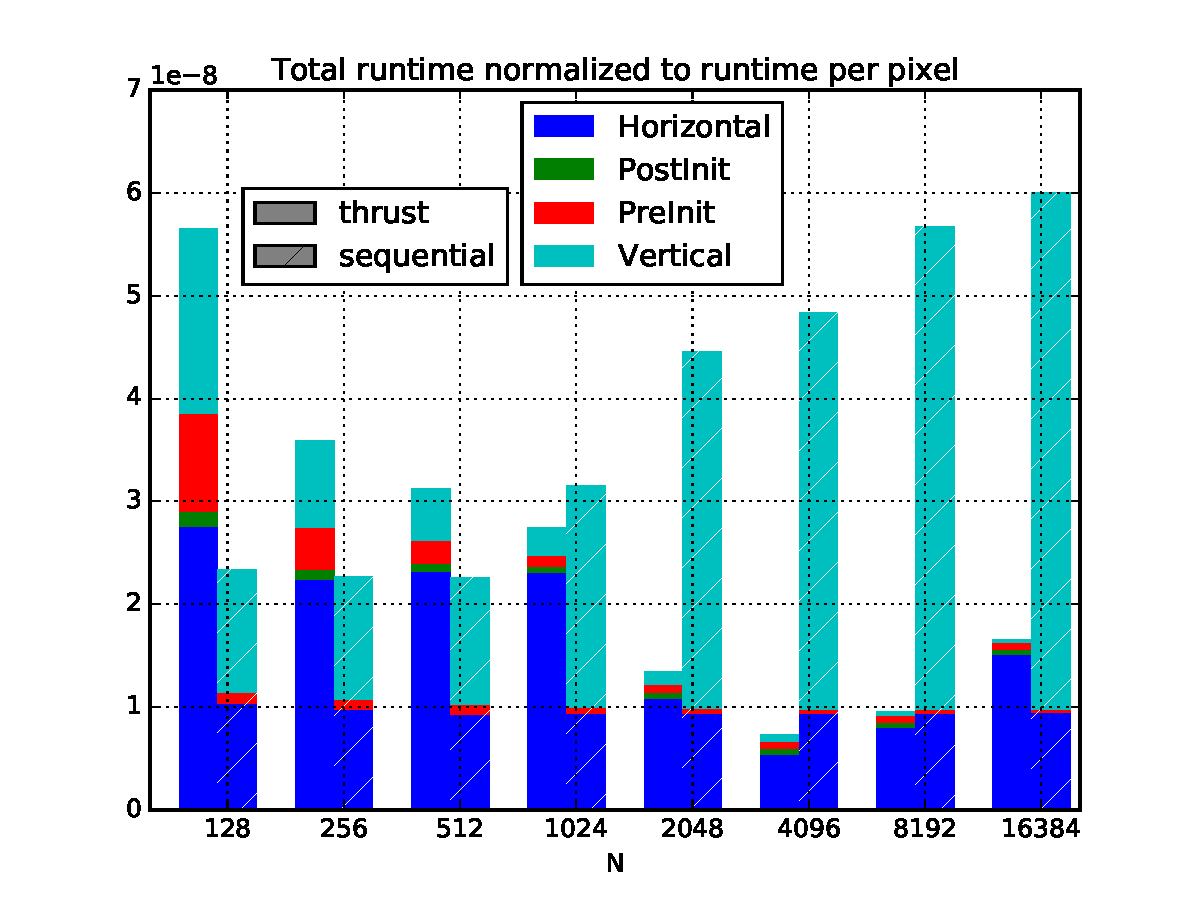
\includegraphics[scale=0.4]{imgs/thrust_vs_sequential_normalized.pdf} 
    \end{column}
    \begin{column}{5cm}
      \begin{itemize}
        \item Initialization and data transfer not limiting
        \item Sequential version's performance degrades for the vertical
          pass - stride causes cache misses
        \item Thrust version is limited by performance of horizontal pass -
          results in non-coalesced memory access (consecutive threads access
          strided data)
      \end{itemize}
    \end{column}
  \end{columns}
\end{frame} 

\subsection{Parallelizing causal and anti-causal pass}
\begin{frame}[fragile]
\frametitle{Parallelizing causal and anti-causal pass}
Just run them on two different streams!
  \begin{lstlisting}[basicstyle=\tiny]
thrust::for_each_n(
  thrust::cuda::par.on(stream),
  thrust::counting_iterator<int>(0), height,
  ...
  \end{lstlisting}
  \begin{figure}
      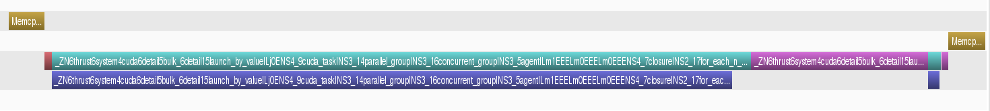
\includegraphics[scale=0.3]{imgs/overlap.png} 
  \end{figure}
  Improves performance but horizontal pass is still the bottleneck.
\end{frame}

\begin{frame}[fragile]
  \frametitle{Combining causality passes}
  \begin{itemize}
    \item Synchronize streams
    \item Add causal and anticausal buffers into result
  \end{itemize}
  Remember: Anticausal pass goes from right to left - yet the original
  implementation writes into the buffer from left to right:
  \begin{lstlisting}[basicstyle=\tiny]
for(int i = 4; i < width; ++i) {
  row[i * column_stride] =
    c.b_anticausal[1] * src[((width - 1) - i + 1) * column_stride]
  + c.b_anticausal[2] * src[((width - 1) - i + 2) * column_stride]
  + c.b_anticausal[3] * src[((width - 1) - i + 3) * column_stride]
  + c.b_anticausal[4] * src[((width - 1) - i + 4) * column_stride]
  - c.a[1] * row[(i - 1) * column_stride]
  - c.a[2] * row[(i - 2) * column_stride]
  - c.a[3] * row[(i - 3) * column_stride]
  - c.a[4] * row[(i - 4) * column_stride];
}
  \end{lstlisting}
\end{frame}

\begin{frame}[fragile]
  \frametitle{Combining causality passes}
  $\implies$ need to reverse anticausal buffer in each row:
  \begin{lstlisting}[basicstyle=\tiny]
cudaStreamSynchronize(s1);
cudaStreamSynchronize(s2);
thrust::for_each_n(
  thrust::counting_iterator<int>(0), height,
  [...] __device__ (int n) {
    auto dest = dest_begin + n * row_stride;
    auto row_l = buffer_l_begin + n * row_stride;
    auto row_r = buffer_r_begin + n * row_stride;
    for(int i = 0; i < width; ++i) {
      dest[i * column_stride] =
      row_l[i * column_stride] + row_r[(width - 1 - i) * column_stride];
    }
  });
  \end{lstlisting}
  Instead, write buffer from right to left and perform fully parallel
  summation:
  \begin{lstlisting}[basicstyle=\tiny]
thrust::transform(
  buffer_l_begin, buffer_l_begin + width * height,
  buffer_r_begin,
  dest_begin,
  thrust::plus<T>());
  \end{lstlisting}
\end{frame}

\subsection{Improving memory access patterns}
\begin{frame}[fragile]
  \frametitle{Horizontal and Vertical memory access patterns}
  Horizontal pass:
  \begin{itemize}
    \item Parallelized over rows
    \item Two threads working on consecutive rows access strided data
    \item $\to$ wasted memory bandwidth
  \end{itemize}

  Vertical pass:
  \begin{itemize}
    \item Parallelized over columns
    \item Two threads working on consecutive columns access consecutive data
    \item $\to$ fully coalesced memory access
  \end{itemize}
\end{frame}

\begin{frame}[fragile]
  \frametitle{Idea to improve access pattern}
  Transpose data instead of performing horizontal pass.
  \begin{enumerate}
    \item Vertical pass
    \item Transpose
    \item Vertical pass
    \item Transpose
  \end{enumerate}
  But:
  \begin{itemize}
    \item Two additional transpose operations which are non-trivial to
      implement efficiently on GPUs
    \item Additional buffer for transpose operation required
    \item Assumes either column-major storage or it works on image mirrored
      along diagonal
  \end{itemize}
\end{frame}

\begin{frame}[fragile]
  \frametitle{Even better}
  \begin{itemize}
    \item Even with a simple thrust implementation this achieves speedups
    \item We can avoid the additional buffer by performing the transposition
      during the addition of the causality buffers
    \item Exactly this, adding two transposed matrices, is also implemented
      in cublas!
  \end{itemize}
  \begin{lstlisting}[basicstyle=\tiny]
T* buffer_l_ptr  = thrust::raw_pointer_cast(&*buffer_l_begin);
T* buffer_r_ptr  = thrust::raw_pointer_cast(&*buffer_r_begin);
T* dest_ptr = thrust::raw_pointer_cast(&*dest_begin);
T alpha = beta = 1.;
cublasSgeam(
  *handle, CUBLAS_OP_T, CUBLAS_OP_T, height, width,
  &alpha, buffer_l_ptr, width,
  &beta, buffer_r_ptr, width,
  dest_ptr, height);
  \end{lstlisting}
\end{frame}

\section{Results} 
\begin{frame}{Performance evaluation}
  The following evaluations were performed on a:
  \begin{itemize}
    \item NVIDIA GeForce GTX 980M
    \item Compute Capability 5.2
  \end{itemize}
  and a:
  \begin{itemize}
    \item Intel Core i7-4810MQ @ 2.8 Ghz
    \item Boost up to 3.8 Ghz
  \end{itemize}
\end{frame} 

\begin{frame}{Times}
  \begin{columns}
    \begin{column}{7cm}
      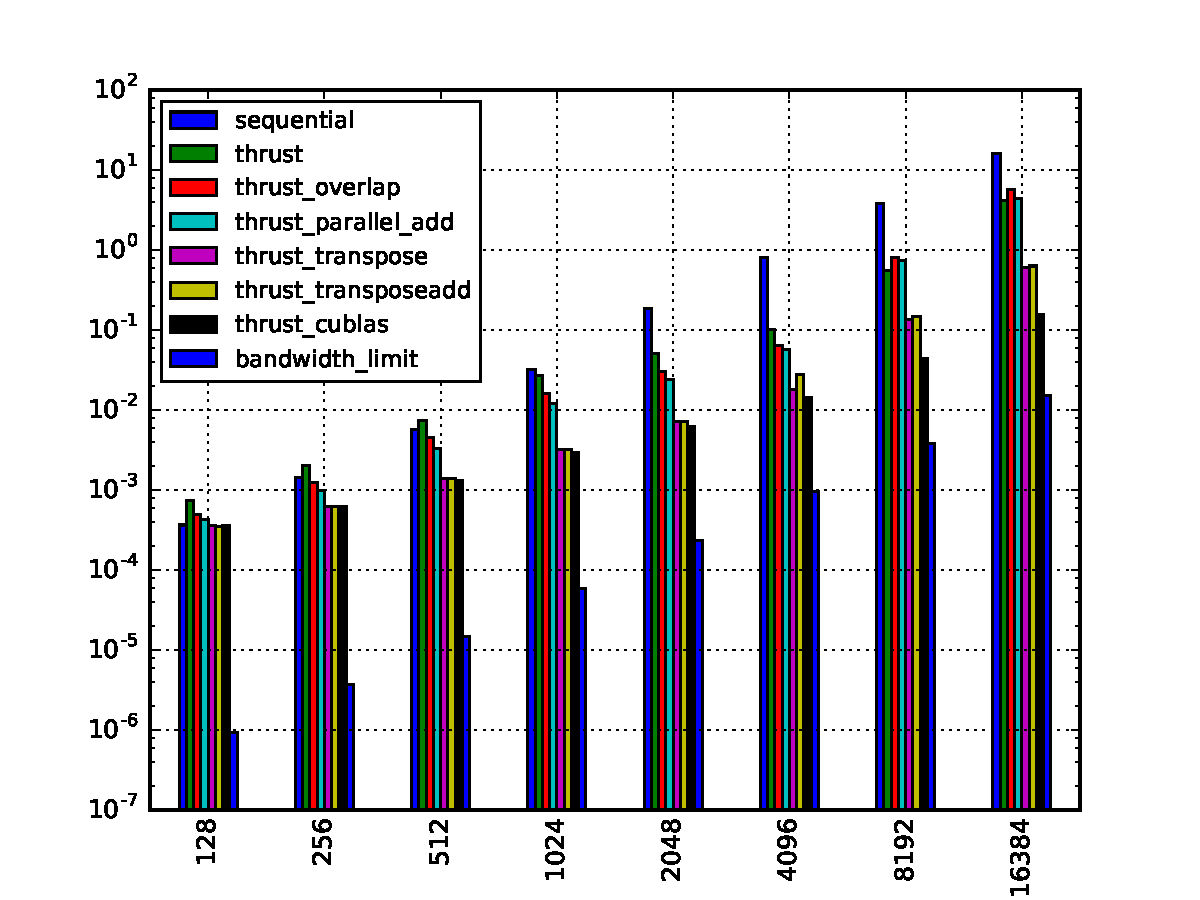
\includegraphics[scale=0.4]{imgs/all_times.pdf} 
    \end{column}
    \begin{column}{3cm}
      \begin{itemize}
        \item Improving memory access most important factor
        \item Optimized cuBLAS geam gives additional boost for larger data
      \end{itemize}
    \end{column}
  \end{columns}
\end{frame} 

\begin{frame}{Speedups}
  \begin{columns}
    \begin{column}{7cm}
      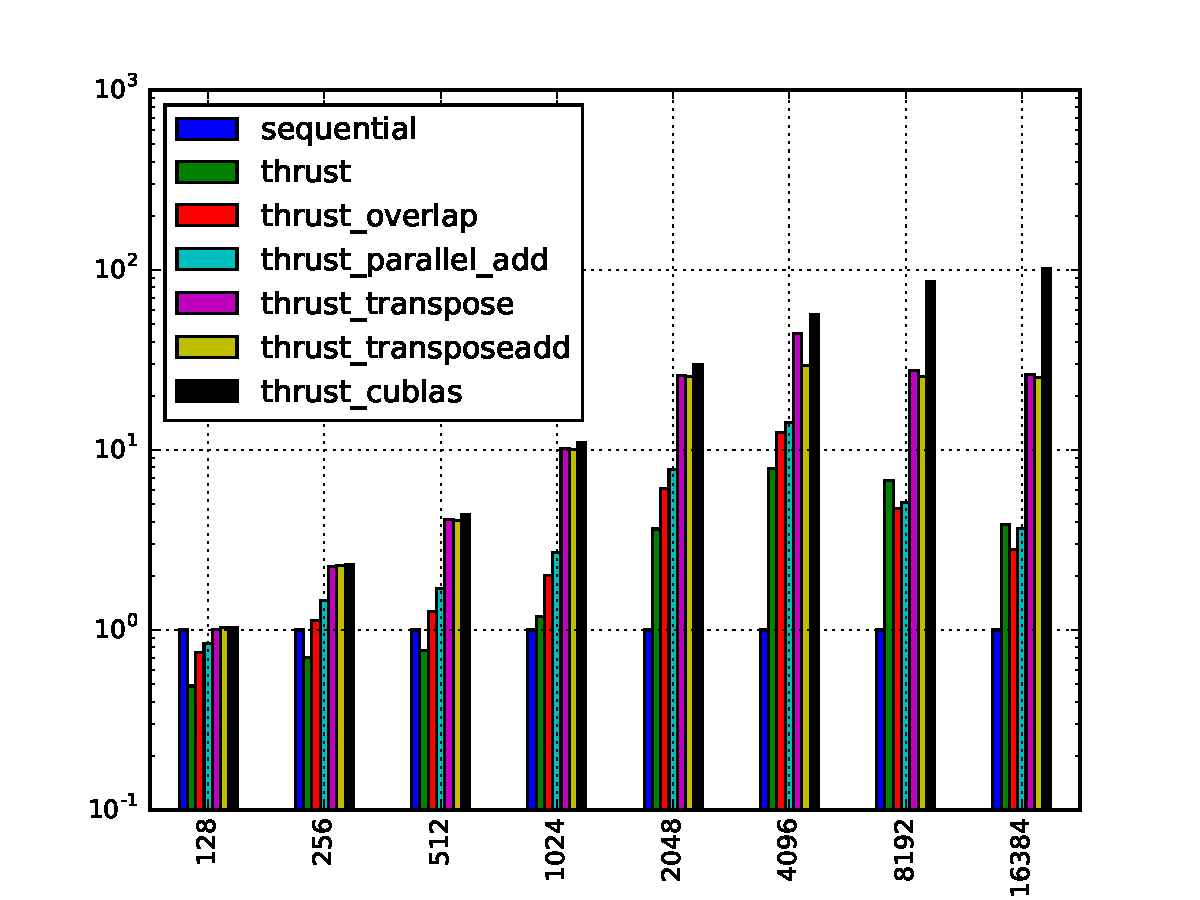
\includegraphics[scale=0.4]{imgs/all_speedups.pdf} 
    \end{column}
    \begin{column}{3cm}
      \begin{itemize}
        \item Maximum speedup of $100$
        \item For $1024x1024$ images: Speedup of $11$ without transfers and $7$ with.
\item $360$ FPS @ $1024x1024$
      \end{itemize}
    \end{column}
  \end{columns}
\end{frame} 


\frame{\frametitle{Further considerations}
Different data and applications need different optimizations.
Here: Image sequences of approximately 1024x1024 pixels.
\begin{itemize}
	\item Parallelization of higher order recurrence relations is more complicated (because prefix sum operators are required to be associative for parallelization) \cite{blelloch1990prefix}
	\item It must be evaluated whether a parallelization of the recurrence relation
		within rows pays off for the relatively small number of $1024$ elements.
  \item Multiple features can be calculated concurrently.
  \item Features of multiple images (from a video sequence) can be calculated concurrently.
  \item Thrust implementation can also run on different backends - e.g.
    OpenMP
\end{itemize}
}

%\begin{frame}[t, allowframebreaks]
\begin{frame}[t]
  \frametitle{References}
  \bibliographystyle{amsalpha}
  \bibliography{doc.bib}
\end{frame}

\end{document}
